\documentclass[12pt,a4paper]{article}
\usepackage[utf8]{inputenc}
\usepackage[T1]{fontenc}
\usepackage[french]{babel}
\usepackage{graphicx}
\usepackage{url}
\usepackage{hyperref}
\usepackage{setspace}
\usepackage{geometry}
\usepackage{caption}
\usepackage{wrapfig}
\usepackage[style=numeric,sorting=none,backend=biber]{biblatex}

\geometry{margin=2.5cm}
\setlength{\intextsep}{6pt}
\setlength{\columnsep}{10pt}
\captionsetup[figure]{font=small}
\addbibresource{rapport.bib}

\title{\textbf{Les rêves à la lumière de l’informatique :\\ entre neurosciences et intelligence artificielle}}
\author{AZZOUZ Ilhem\\BELKACEMI Cirine\\BOURAKKADI IDRISSI Marwa}
\date{Le 24 Novembre}

\begin{document}
\maketitle
\tableofcontents
\newpage

\section{Introduction}
On appelle rêve « tout contenu mental qui se produit pendant le sommeil », explique Delphine Oudiette, chercheuse à l’Institut du Cerveau (ICM). Cela va de la simple pensée aux élaborations les plus oniriques, selon le stade et l’avancée de la nuit. Comme le rappelle Claudia Picard-Deland : « On peut recueillir des rêves chez les dormeurs à tout moment du cycle du sommeil. »  
Aujourd’hui, grâce aux progrès de l’informatique et de l’intelligence artificielle, il devient possible d’étudier, de simuler, voire d’interpréter les rêves d’une manière inédite.  

Ce rapport explore la relation entre le monde onirique et l’informatique moderne : comment les technologies numériques permettent de mieux comprendre les rêves, de modéliser les processus cérébraux associés et d’ouvrir la voie à de nouvelles applications.

\section{Les rêves : une perspective scientifique}

\begin{wrapfigure}{r}{0.28\textwidth}
\vspace{-\baselineskip}
\centering
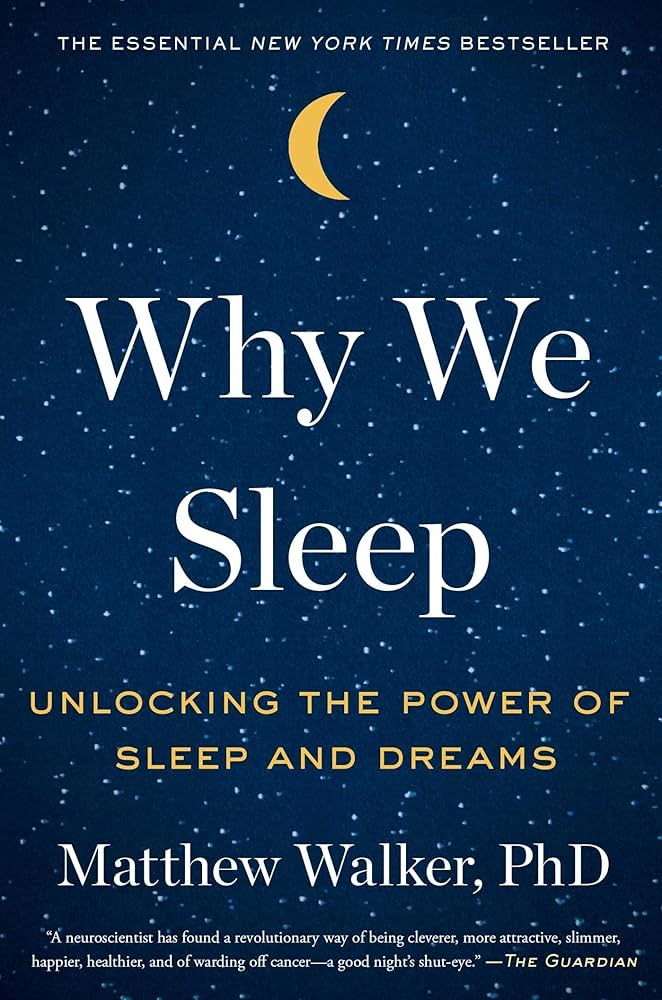
\includegraphics[width=0.2\textwidth]{why_we_sleep_cover.jpg}
\caption{Couverture de \textit{Why We Sleep} (M. Walker)}
\end{wrapfigure}

Les rêves sont des phénomènes mentaux qui surviennent principalement durant la phase de sommeil paradoxal (REM).  
Le cerveau y manifeste une activité électrique intense, proche de l’état d’éveil.  
Les neurosciences utilisent aujourd’hui l’imagerie cérébrale (IRMf, EEG) pour étudier les zones du cerveau actives pendant le rêve.  
Ces données constituent une base essentielle pour l’analyse informatique et la modélisation.  

Comme le décrit Matthew Walker dans son ouvrage \textit{Why We Sleep}~\cite{walker} :  
« Le rêve est une sorte de laboratoire de simulation émotionnelle où le cerveau rejoue les expériences du jour pour mieux les comprendre et les intégrer. »

\section{Informatique et étude des rêves}
Les technologies informatiques jouent un rôle clé dans la recherche sur le rêve :  
\begin{itemize}
    \item \textbf{Acquisition de données} : des capteurs EEG enregistrent l’activité cérébrale, ensuite traitée par des algorithmes.  
    \item \textbf{Traitement du signal} : les logiciels analysent les ondes cérébrales pour identifier les phases de sommeil.  
    \item \textbf{Apprentissage automatique} : des modèles d’IA cherchent à prédire les contenus ou émotions des rêves à partir de signaux physiologiques.  
\end{itemize}

Dans un reportage diffusé sur Arte intitulé \textit{Les rêves dévoilés}~\cite{arte}, les chercheurs montrent comment des algorithmes d’intelligence artificielle peuvent « traduire » les signaux neuronaux en images approximatives de ce que le dormeur imagine.  
Ces approches rapprochent les sciences cognitives et l’intelligence artificielle.

\section{La simulation des rêves par l’intelligence artificielle}
L’intelligence artificielle, notamment les réseaux de neurones génératifs (GANs), peut produire des images, des sons ou des scénarios qui ressemblent à des rêves.  
Selon un article de Polytechnique Insights~\cite{polytechnique} :  
« Des progrès récents dans le domaine du Machine Learning et de la neuroimagerie ont aidé les chercheurs à identifier certains schémas d’activité cérébrale liés aux rêves. »  

Des outils comme \textit{DeepDream} de Google utilisent des réseaux neuronaux pour créer des visions oniriques à partir d’images réelles~\cite{itsmf}.  
Dans le documentaire \textit{In Your Mind: Decoding Dreams with AI}~\cite{bbc}, on voit comment des modèles IA transforment des signaux cérébraux en images floues rappelant les rêves du dormeur.  

Ces systèmes “rêvent” au sens figuré : ils explorent des combinaisons nouvelles d’informations internes.  
Ce parallèle entre le rêve humain et le rêve artificiel ouvre des perspectives fascinantes pour la compréhension de la créativité et de la conscience.

\section{Applications concrètes}
Les recherches informatiques sur les rêves trouvent des applications dans :
\begin{itemize}
    \item la médecine du sommeil (détection automatique des troubles du sommeil) ;
    \item la psychologie (analyse assistée par IA des contenus oniriques pour la thérapie) ;
    \item l’art numérique (création d’œuvres inspirées des rêves générés par IA) ;
    \item les interfaces cerveau-machine (décodage des signaux cérébraux pendant le sommeil).
\end{itemize}

Un exemple notable est le projet « Brain2Image » de l’université de Kyoto, où les chercheurs ont réussi à reconstituer des images mentales à partir de signaux IRMf, ouvrant la voie à des applications thérapeutiques inédites.

\section{Limites et enjeux éthiques}
Malgré les avancées, l’étude informatique des rêves soulève des défis :  
\begin{itemize}
    \item la protection de la vie privée, car les signaux cérébraux sont extrêmement personnels ;  
    \item les questions éthiques : peut-on “lire” ou interpréter les pensées d’une personne sans son accord ?  
    \item la fiabilité : les algorithmes actuels ne reproduisent pas encore la complexité émotionnelle des rêves humains.  
\end{itemize}

Comme le souligne le philosophe Jean-Michel Besnier dans \textit{Demain les posthumains}~\cite{besnier} :  
« À force de vouloir pénétrer l’intime du rêve, l’homme risque d’oublier ce qu’il a de plus précieux : le mystère de sa propre conscience. »

\section{Conclusion}
Les rêves, longtemps perçus comme un mystère inaccessible, deviennent aujourd’hui un champ d’étude interdisciplinaire où l’informatique joue un rôle central.  
Des outils d’analyse, de simulation et de génération de rêves artificiels permettent d’explorer la frontière entre la biologie, la conscience et la machine.  
À l’avenir, la convergence entre neurosciences et intelligence artificielle pourrait nous permettre non seulement de comprendre nos rêves, mais aussi d’en créer de nouveaux.

\newpage
\printbibliography

\end{document}
